% =====================================================================================================
\section{Further Experiments}\label{sec:further}
\subsection{Bitrate regulation}
\begin{figure}[t]
\centering
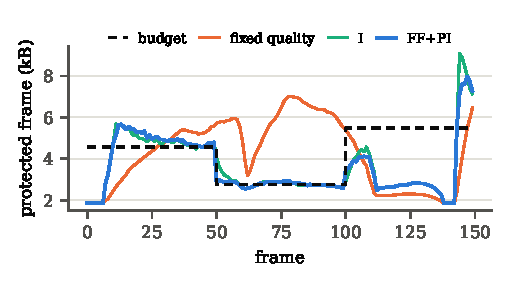
\includegraphics[width=\columnwidth]{figures/fig_rate_control.pdf}
\caption{Bitrate regulation on the Sintel trailer: protected frame size under a budget that follows the link (100\,\%, 60\,\%, 120\,\% of the clip's median), with fixed quality, integral control and feed-forward plus PI.}
\label{fig:rc}
\end{figure}
A sender on a shared link must follow the available bandwidth $B_k$. Treating the quality factor like the voltage of a motor drive, we compared fixed quality, bang-bang, integral, PI and feed-forward plus PI control (Fig.~\ref{fig:rc}). JPEG maps quality $q$ to the scale of the quantization tables as $5000/q$ below 50 and $200 - 2q$ above, so one quality step changes the bytes about four times more at low quality than at high quality; the controllers therefore act on $u = \ln(\text{scale})$, in which the plant is nearly linear, $\ln S_k \approx a - g\,u_k$, and on the logarithmic error
\begin{equation}
\varepsilon_k = \ln (B_k / S_k),
\label{eq:rcerr}
\end{equation}
which is symmetric (twice too big counts as much as half too small). The PI law in velocity form, with a slew limit $|\Delta u| \le \Delta_{\max}$, is
\begin{equation}
\begin{aligned}
\Delta u_k &= K_P (\varepsilon_k - \varepsilon_{k-1}) + K_I \varepsilon_k,\\
u_{k+1} &= u_k - \operatorname{clip}(\Delta u_k, \pm\Delta_{\max}),
\end{aligned}
\label{eq:pi}
\end{equation}
and the feed-forward term jumps by $\Delta u = -\ln(B_{k}/B_{k-1})/\hat g$ when the budget changes, with $\hat g$ estimated online by recursive least squares while the input is excited. After settling, fixed quality misses the budget by \RcFixedErrMin--\RcFixedErrMax\,\% on \RcClips{} real clips, integral control by \RcIErrMin--\RcIErrMax\,\% and feed-forward plus PI by \RcFfpiErrMin--\RcFfpiErrMax\,\%, which settles within \RcFfpiSettleMax{} frames of a bandwidth drop (\RcSynFfpiErr\,\% on the synthetic scene). Scene cuts are disturbances that no causal controller anticipates. A controller tuned in the quality domain oscillated at low quality on one clip; acting on $u$ keeps the loop gain nearly constant over the whole range.

\subsection{Change-driven coding}
\begin{figure}[t]
\centering
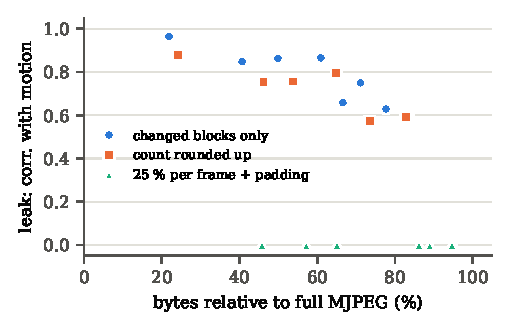
\includegraphics[width=\columnwidth]{figures/fig_change_driven.pdf}
\caption{Change-driven coding: bytes against the leak of motion (the larger correlation of the per-frame block count or frame size with the true motion) for three policies, one point per source. Only coding a constant share of blocks and padding every frame hides motion.}
\label{fig:change}
\end{figure}
Coding only the 16$\times$16 blocks that changed, as a retina does, needs \CdBytesFixed\,\% of the bytes on the fixed camera but \CdBytesMin--\CdBytesMax\,\% on the real clips, and the number of coded blocks tracks motion (correlation \CdCountFixed{} and \CdCountMin--\CdCountMax) even when the change map is hidden (Fig.~\ref{fig:change}). Coding a constant 25\,\% of the blocks per frame, refreshing the oldest unchanged ones, and padding every frame hides both, at \CdPadFixed\,\% of the bytes and SSIM \CdPadSsimFixed{} on the fixed camera, but SSIM falls to \CdPadSsimMin--\CdPadSsimMax{} on edited clips.

\subsection{Keyed block transforms}
Independent keyed flips per block defeat jigsaw solvers for block-scrambling ciphers. For the DCT, a flip is a pattern of sign changes, which E5 already encrypts: on \BtSources{} sources the jigsaw solver stays at chance (at most \BtNbMax\,\% neighbours) with or without keyed flips, and even with every tile position given, SSIM changes by at most \BtSsimDelta. E5's protection therefore rests on the block positions; an attacker who knew them would reach SSIM \BtOracleMin--\BtOracleMax{} on the real clips (\BtOracleFixed{} on the synthetic scene).
